\section{Eksperimen dan Analisis}

\subsection{Rancangan Eksperimen}

\subsubsection{Data Training dan Data Test}

Berkas \texttt{train.csv} berisi 27.373 pemesanan berlabel dengan 17 fitur (14
numerik dan 3 kategorikal), sedangkan \texttt{test.csv} tidak berlabel dan hanya
dipakai untuk menghasilkan prediksi \textit{submission}. Kedua berkas diproses
terpisah, yaitu seluruh parameter \textit{preprocessing} dipelajari dari data
latih lalu diterapkan pada data uji tanpa digabung.

Sekitar 67\% pemesanan pada data latih tidak dibatalkan sehingga akurasi
\textit{baseline} sudah 0,675 dan evaluasi perlu memakai \textit{Macro F1}.
\texttt{days\_before\_arrival} paling berkorelasi dengan pembatalan ($0{,}44$)
sehingga makin jauh hari pemesanan dibuat, makin besar peluang batal, sedangkan
\texttt{special\_requests} berkorelasi negatif ($-0{,}26$). Dari fitur
kategorikal, \texttt{booking\_channel} paling membedakan, yaitu \textit{Online Travel Agent} paling sering batal (36\%), \textit{Corporate} jarang (12\%), dan
\textit{Complimentary} tidak pernah batal. Pembatalan juga berubah mengikuti
bulan, misalnya sekitar 47\% pada Agustus sampai Oktober 2024 tetapi hanya 3\%
pada Januari 2024.

\subsubsection{Pembagian Data dan Validasi}

Pembagian data memakai \texttt{StratifiedGroupKFold} dengan 5 \textit{fold},
\textit{seed} 42, dan pengacakan. Stratifikasi menjaga proporsi kelas batal
sekitar 33\% pada tiap \textit{fold}, sedangkan pengelompokan menjaga baris yang
identik tetap berada pada satu sisi pembagian. Fold pertama (20\% data) dipakai sebagai
data validasi untuk memilih konfigurasi tiap model, dan seluruh model memakai
fold yang sama agar hasilnya sebanding. Evaluasi akhir memakai \textit{5-fold cross-validation} penuh dengan
seluruh langkah \textit{preprocessing} dan pelatihan diulang pada tiap
\textit{fold}, dan hasilnya dilaporkan sebagai rata-rata dan simpangan baku.
Model akhir untuk \textit{submission} dilatih ulang pada seluruh \texttt{train.csv}.

\subsubsection{Konfigurasi Parameter}

Tabel~\ref{tab:param} merangkum konfigurasi terpilih tiap model. Nilai tersebut
dipilih pada data validasi, kecuali faktor \textit{oversampling} C4.5 yang
dipilih dengan validasi silang di dalam data latih.

\begin{table}[H]
\centering
\small
\caption{Konfigurasi terpilih tiap model}
\label{tab:param}

\begin{tabularx}{\textwidth}{@{}lX@{}}
\toprule
Model & Konfigurasi \\
\midrule
KNN & Standardisasi, $k=31$, bobot \texttt{distance} \\
C4.5 & \textit{Gain ratio}, \textit{Reduced Error Pruning} (80\% data pembentuk pohon dan 20\% data \textit{pruning}), \textit{oversampling} kelas batal 2,0 kali, tanpa imputasi, ditambah fitur turunan \\
\textit{Logistic Regression} & \textit{Gradient ascent}, $\lambda=0{,}001$, laju belajar 0,1 \\
SVM & SMO dengan kernel linear, dilatih pada 1.000 baris karena matriks kernel penuh membutuhkan memori $O(n^2)$ \\
\textit{Naive Bayes} & \textit{Binning} 20 kuantil untuk fitur kontinu, $\alpha=2$ \\
\bottomrule
\end{tabularx}
\end{table}

\subsubsection{Metrik Evaluasi}

Metrik dihitung dengan \texttt{sklearn.metrics} dari \textit{confusion matrix}.

\begin{itemize}
    \item \textit{Macro F1} adalah metrik utama, sama dengan metrik
        \textit{leaderboard} Kaggle. Metrik ini merata-ratakan $F_1$ kelas batal
        dan tidak batal sehingga kedua kelas berbobot sama.
    \item \textit{Accuracy}, \textit{precision}, \textit{recall}, dan $F_1$ kelas
        batal sebagai pelengkap. \textit{Accuracy} dibandingkan dengan
        \textit{baseline} 0,675 yang diperoleh jika semua pemesanan ditebak
        tidak batal.
    \item \textit{ROC-AUC} menilai kualitas urutan probabilitas tanpa bergantung
        pada satu \textit{threshold}. Pada C4.5 probabilitas diambil dari
        proporsi kelas pada daun.
    \item \textit{Log-loss} dipakai untuk membandingkan \textit{Logistic Regression} dengan \texttt{scikit-learn}.
\end{itemize}

Selain metrik prediksi, implementasi sendiri dibandingkan dengan
\texttt{scikit-learn} menggunakan metrik yang sama, selisih probabilitas
prediksi, jumlah node pohon, dan waktu pelatihan. Untuk bonus
\textit{cost-sensitive}, ukuran utamanya adalah total biaya
$2\times FP+1\times FN$ dan biaya per pemesanan, dihitung dari prediksi
\textit{out-of-fold} sehingga tiap pemesanan dievaluasi oleh model yang tidak
melatihnya.

\subsection{Hasil Eksperimen dan Visualisasi}

\subsubsection{K-Nearest Neighbors}

Setiap kombinasi skema \textit{scaling}, nilai $k$, dan bobot dievaluasi pada
data validasi. Bobot \texttt{distance} selalu sama atau lebih baik daripada
\texttt{uniform}. Pada bobot \texttt{uniform}, F1 macro turun menjadi sekitar
0,79 saat $k=51$, sedangkan pada \texttt{distance} tetap sekitar 0,83 sampai
0,84 karena tetangga yang jauh hanya mendapat suara kecil. Standardisasi dengan
$k=31$ memberi F1 macro tertinggi (0,841), sedikit di atas \textit{min-max}
(0,838 pada $k=11$), sedangkan transformasi log paling buruk karena
memperkecil perbedaan lead time dan harga yang justru menjadi sinyal kuat.

\subsubsection{Decision Tree Learning}

Pohon C4.5 tanpa \textit{pruning} tumbuh sangat besar karena fitur turunan
menambah banyak kandidat ambang, dengan F1 macro hanya 0,800. \textit{Reduced Error Pruning} memangkasnya menjadi 9.764 simpul dan menaikkan F1 macro menjadi
0,845. Oversampling dua kali lipat menaikkan \textit{recall} dari 0,759 menjadi
0,780 tetapi menurunkan \textit{precision} dari 0,819 menjadi 0,786, sehingga F1
macro sedikit turun menjadi 0,839. Selisih ini masih dalam rentang variasi
antar-\textit{fold} (sekitar 0,01) sehingga oversampling tidak terbukti membantu
maupun merugikan, tetapi tetap dipakai karena faktornya dipilih lewat validasi
silang.

\begin{table}[H]
\centering
\small
\caption{Pengaruh \textit{pruning} dan \textit{oversampling} pada C4.5 (data validasi)}
\label{tab:dtl}

\begin{tabular}{@{}lcc@{}}
\toprule
Konfigurasi C4.5 & Jumlah simpul & F1 macro \\
\midrule
Tanpa \textit{pruning} & 57.264 & 0,800 \\
Dengan \textit{Reduced Error Pruning} & 9.764 & 0,845 \\
Dengan \textit{pruning} dan oversampling & - & 0,839 \\
\bottomrule
\end{tabular}
\end{table}

Pada visualisasi pohon (Gambar~\ref{fig:pohon}), atribut pertama adalah
\texttt{days\_before\_arrival} dengan ambang 148,5 hari, sesuai temuan bahwa
\textit{lead time} paling berhubungan dengan pembatalan. Fitur turunan
\texttt{special\_requests\_missing} juga muncul di level atas.

\begin{figure}[H]
\centering
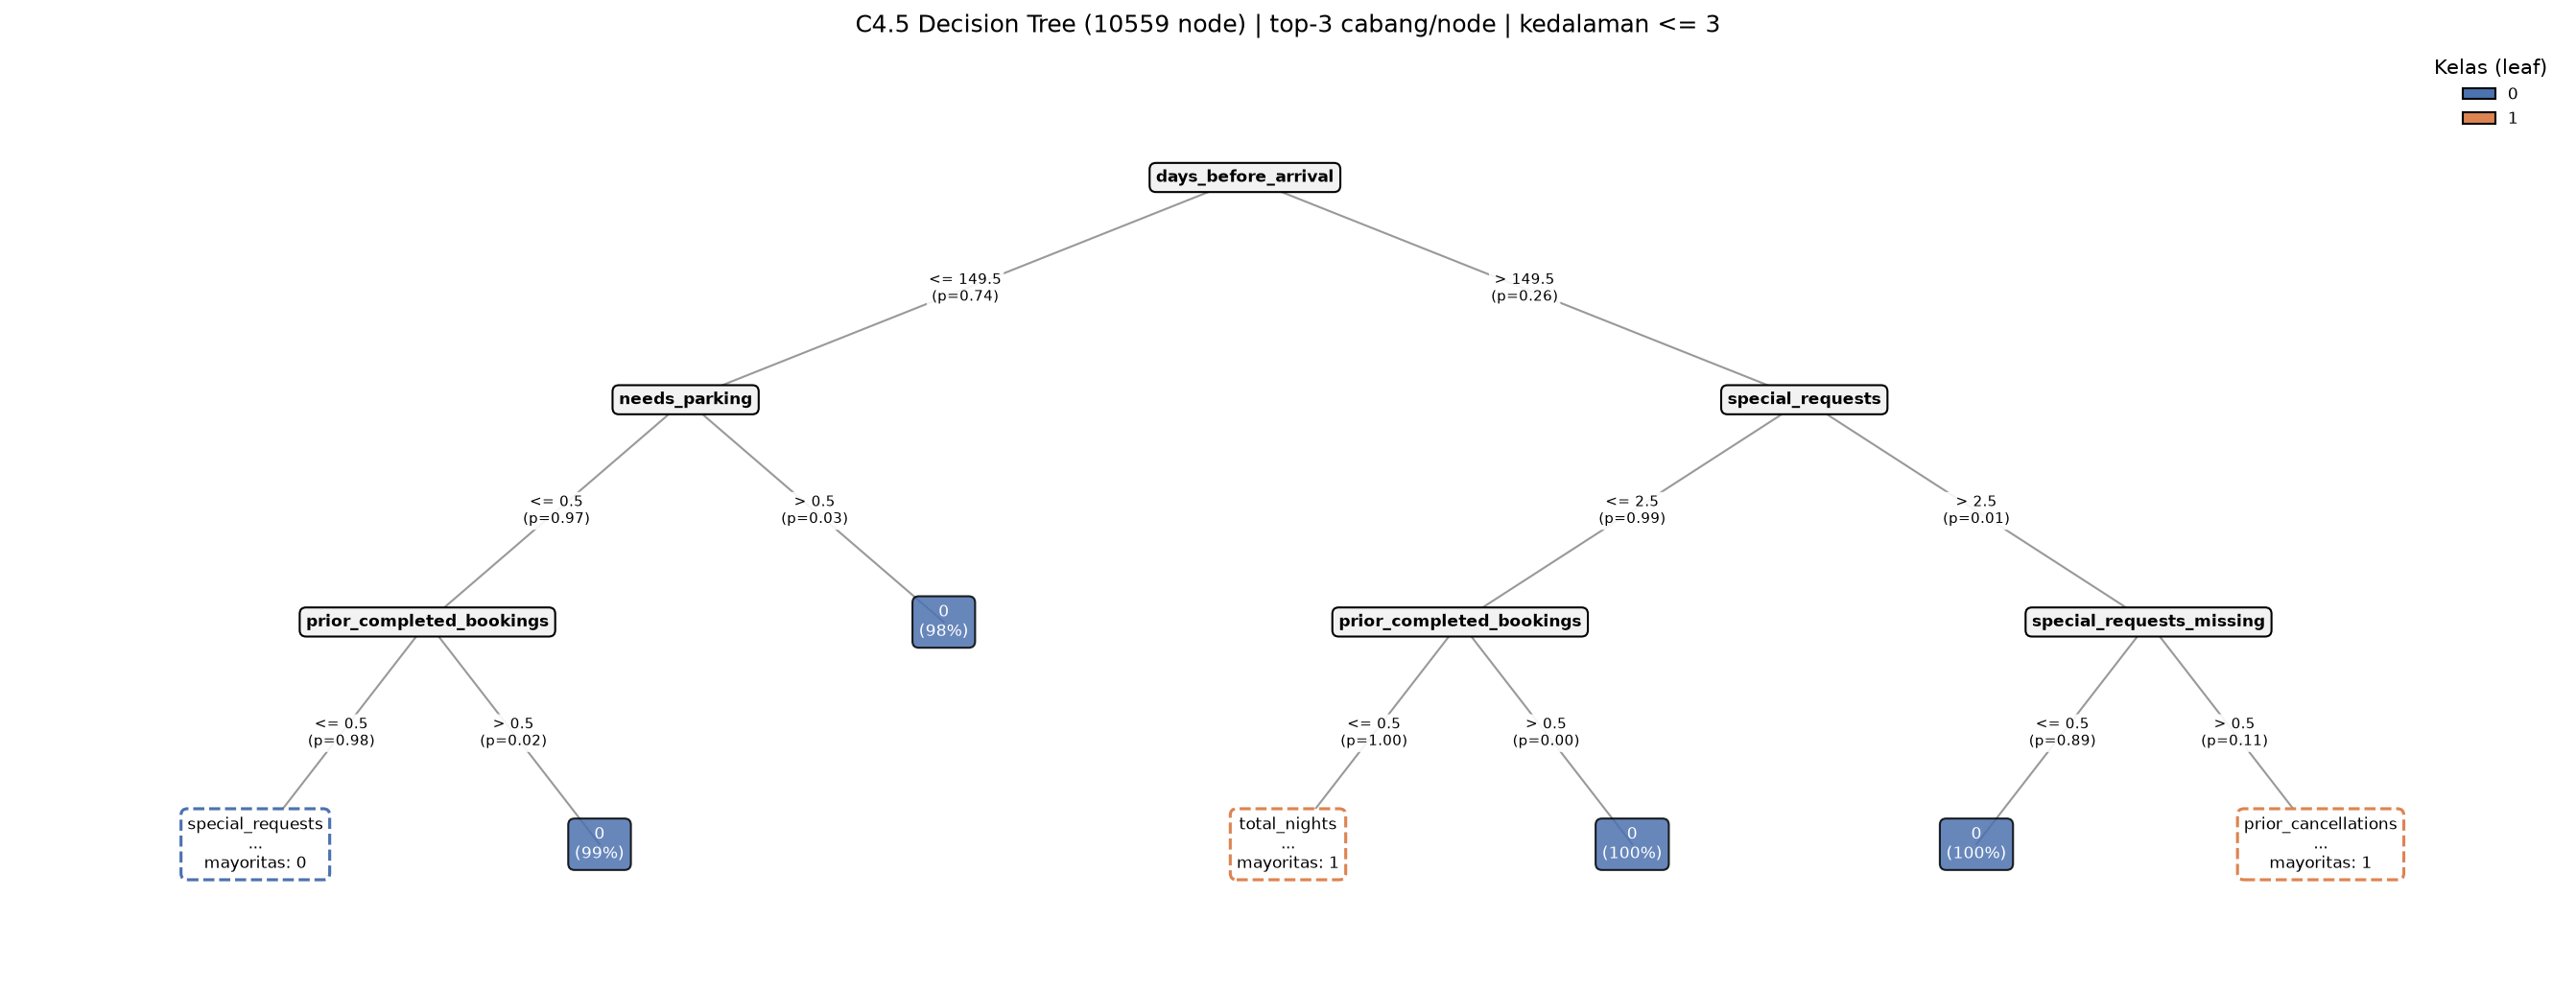
\includegraphics[width=\textwidth]{../output/c45_tree.png}
\caption{Visualisasi tiga level teratas pohon C4.5 (\texttt{top\_n}=3)}
\label{fig:pohon}
\end{figure}

\subsubsection{Logistic Regression}

Empat varian (tanpa penalti, L1, L2, dan \textit{Elastic Net}) dilatih pada
konfigurasi yang setara ($\lambda=0{,}001$). Pengaruh regularisasi sangat kecil
karena $\lambda$ kecil dan data cukup banyak, sehingga keempat varian hampir
tidak berbeda, dengan \textit{accuracy} 0,806 sampai 0,808 dan ROC-AUC 0,865
pada data validasi. Kurva \textit{loss} pelatihan tiap varian ditunjukkan pada
Gambar~\ref{fig:logreg}.

\begin{figure}[H]
\centering
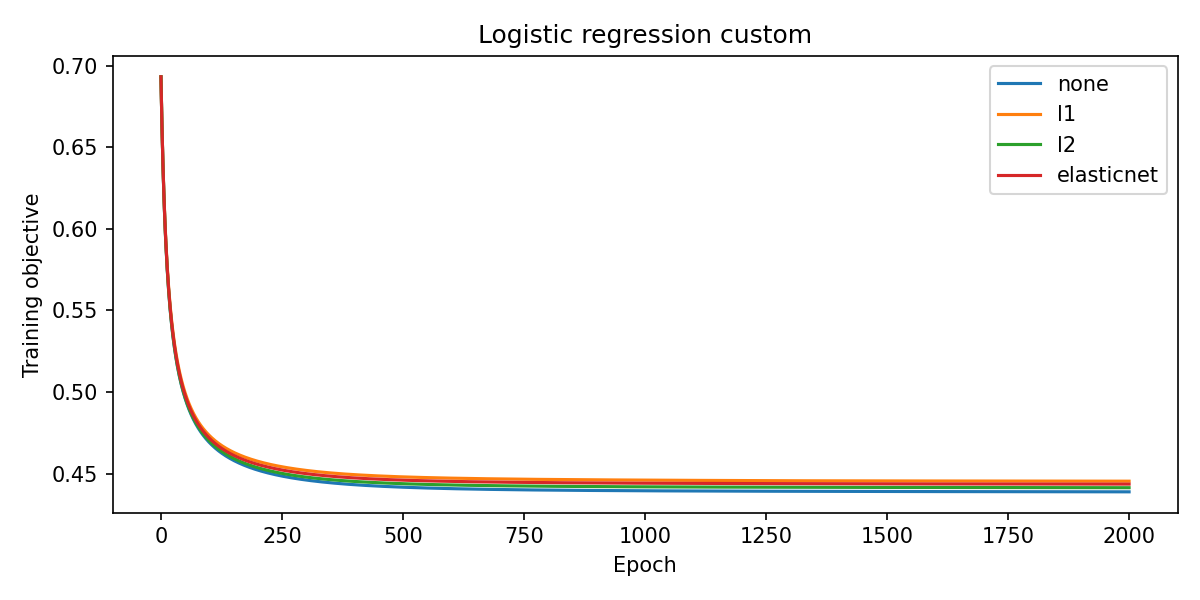
\includegraphics[width=0.8\textwidth]{../output/logreg_loss.png}
\caption{Kurva \textit{loss} pelatihan \textit{Logistic Regression} buatan sendiri}
\label{fig:logreg}
\end{figure}

\subsubsection{Support Vector Machine}
% TODO: Tabel metrik, pengaruh kernel dan C.

\subsubsection{Bayesian Network (Naive Bayes)}
% TODO: Tabel metrik, distribusi probabilitas kelas.

\subsubsection{Perbandingan Antarmodel}

Tabel~\ref{tab:cv} memuat hasil \textit{5-fold cross-validation} dengan
konfigurasi terbaik tiap model.

\begin{table}[H]
\centering
\small
\caption{Hasil \textit{5-fold cross-validation} (rata-rata)}
\label{tab:cv}

\begin{tabular}{@{}lccccc@{}}
\toprule
Model & \textit{Accuracy} & \textit{Precision} & \textit{Recall} & F1 macro & ROC-AUC \\
\midrule
KNN & 0,855 & 0,805 & 0,737 & 0,832 $\pm$ 0,008 & 0,914 \\
C4.5 & 0,853 & 0,795 & 0,744 & 0,830 $\pm$ 0,006 & 0,865 \\
\textit{Logistic Regression} & 0,797 & 0,731 & 0,605 & 0,759 $\pm$ 0,009 & 0,854 \\
SVM & 0,794 & 0,726 & 0,597 & 0,754 $\pm$ 0,010 & 0,843 \\
\textit{Naive Bayes} & 0,781 & 0,687 & 0,610 & 0,744 $\pm$ 0,006 & 0,836 \\
\bottomrule
\end{tabular}
\end{table}

\begin{figure}[H]
\centering
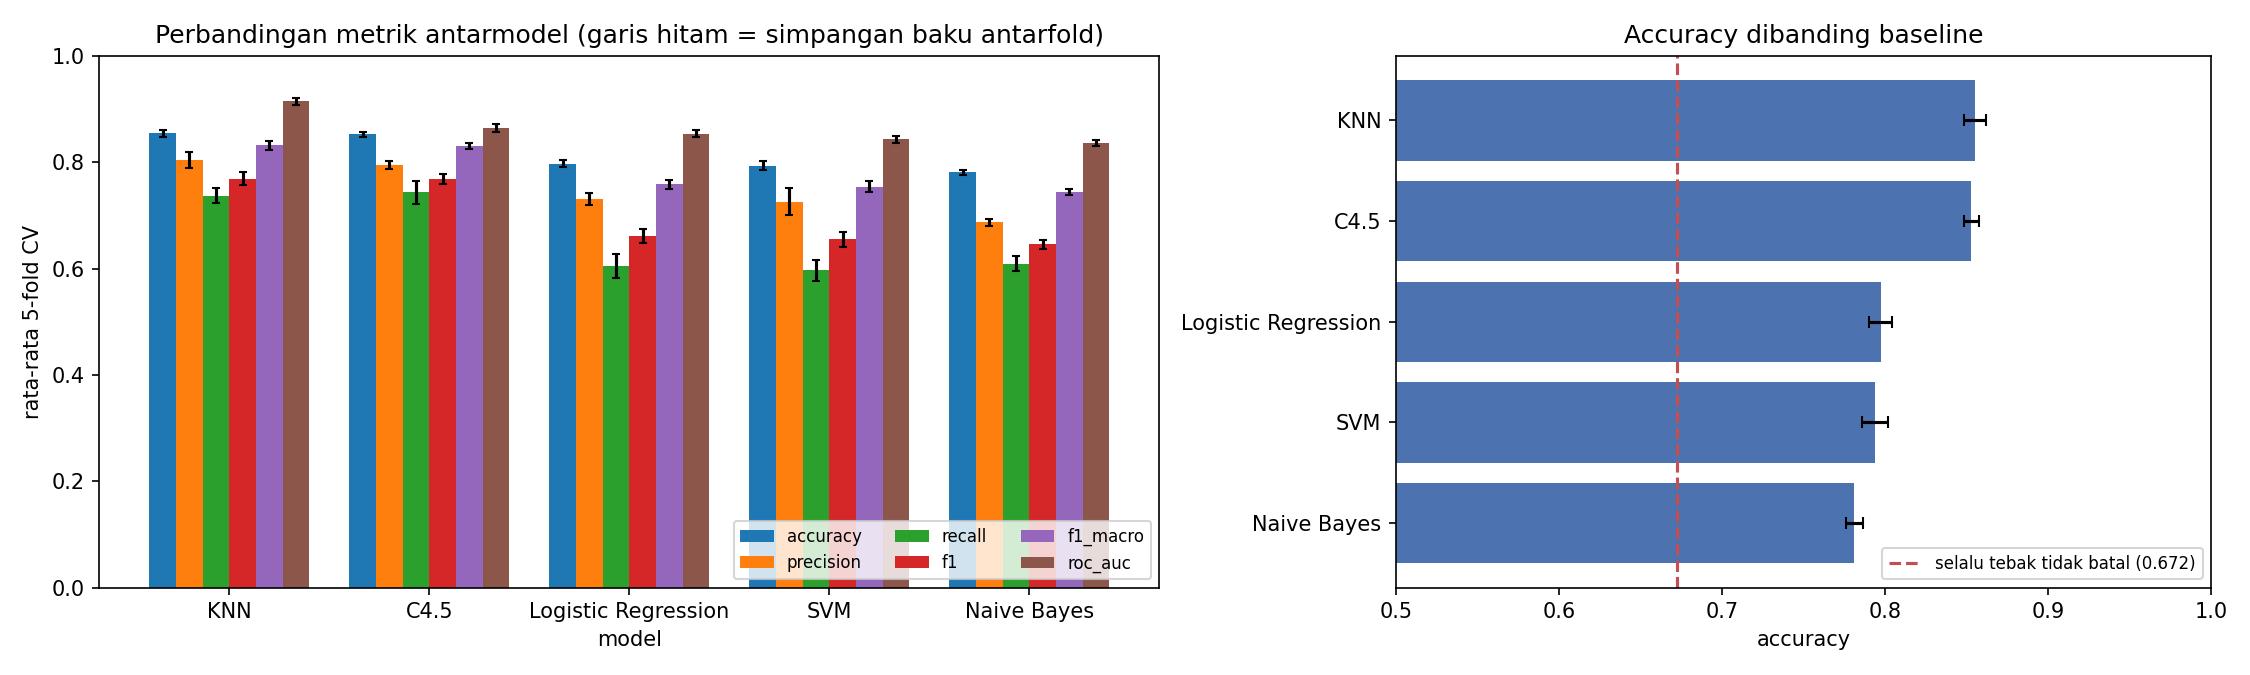
\includegraphics[width=\textwidth]{../output/model_comparison.png}
\caption{Perbandingan metrik antarmodel}
\label{fig:model}
\end{figure}

KNN dan C4.5 memperoleh hasil tertinggi dengan selisih yang jauh lebih kecil dibandingkan
variasi antar-\textit{fold}, sehingga keduanya dapat dianggap setara. Perbedaan
terbesar ada pada ROC-AUC (0,914 untuk KNN dan 0,865 untuk C4.5) karena
probabilitas KNN berasal dari 31 tetangga berbobot jarak sehingga lebih halus,
sedangkan probabilitas C4.5 hanya proporsi kelas pada daun. \textit{Logistic Regression} dan SVM hampir sama karena SVM terbaik memakai kernel linear
sehingga keduanya sama-sama membentuk batas lurus. KNN dan C4.5 unggul karena
dapat menangkap pola nonlinear dan interaksi antarfitur, sedangkan model linear
hanya memberi satu bobot pada tiap fitur. Semua model jauh di atas
\textit{baseline} 0,675, tetapi \textit{recall} hanya 0,60 sampai 0,74
sehingga 26 sampai 40\% pemesanan yang batal belum terdeteksi. Fold pertama
memberi skor tertinggi untuk semua model, kemungkinan karena konfigurasi
dipilih dengan \textit{fold} tersebut, sehingga rata-rata 5 \textit{fold} lebih
dapat dipercaya untuk membandingkan model.

\subsubsection{Cost-Sensitive Classification}

Tabel~\ref{tab:cost} membandingkan prediksi \textit{out-of-fold} pada
\textit{threshold} 0,5 dan 0,667 dengan $C_{FP}=2$ dan $C_{FN}=1$. SVM tidak
disertakan karena skornya bukan probabilitas.

\begin{table}[H]
\centering
\small
\caption{Pengaruh \textit{threshold} \textit{cost-sensitive} terhadap total biaya}
\label{tab:cost}

\begin{tabular}{@{}lcrrr@{}}
\toprule
Model & \textit{Threshold} & $FP$ & $FN$ & Total biaya \\
\midrule
KNN & 0,5 & 1.607 & 2.359 & 5.573 \\
 & 0,667 & 614 & 3.865 & 5.093 \\
C4.5 & 0,5 & 1.722 & 2.299 & 5.743 \\
 & 0,667 & 1.474 & 2.492 & 5.440 \\
\textit{Logistic Regression} & 0,5 & 1.997 & 3.549 & 7.543 \\
 & 0,667 & 839 & 5.311 & 6.989 \\
\textit{Naive Bayes} & 0,5 & 2.488 & 3.503 & 8.479 \\
 & 0,667 & 1.027 & 4.948 & 7.002 \\
\bottomrule
\end{tabular}
\end{table}

Pada semua model, \textit{threshold} 0,667 menurunkan jumlah $FP$ dan menaikkan
jumlah $FN$, dan total biaya ikut turun karena $FP$ berbobot dua kali lipat.
Penurunan terbesar terjadi pada \textit{Naive Bayes} (sekitar 17\%), yang
memiliki $FP$ terbanyak pada \textit{threshold} 0,5, dan terkecil pada C4.5
(sekitar 5\%). KNN memiliki total biaya terendah (5.093), dengan $FP$ turun
dari 1.607 menjadi 614. Perubahan ini memberi pertukaran yang harus
dipertimbangkan, yaitu lebih banyak pemesanan batal yang tidak terdeteksi sebagai
imbalan lebih sedikit risiko \textit{overbooked}.

\begin{figure}[H]
\centering
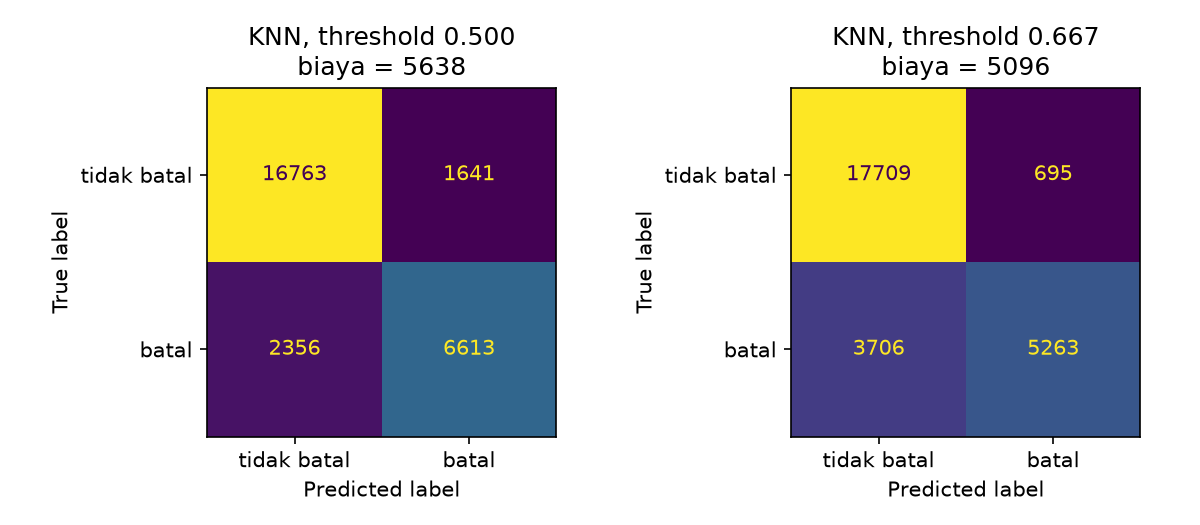
\includegraphics[width=0.8\textwidth]{../output/cost_sensitive_confusion_matrix.png}
\caption{\textit{Confusion matrix} model dengan biaya terendah pada kedua \textit{threshold}}
\label{fig:cost}
\end{figure}

\subsection{Perbandingan Implementasi dengan Pustaka}

\subsubsection{Perbandingan Metrik}

Tiap algoritma dibandingkan dengan padanannya pada \texttt{scikit-learn} pada
data validasi yang sama.

\paragraph{KNN.} Hasil kedua implementasi identik (Tabel~\ref{tab:knn}). Hanya
satu dari 5.474 baris validasi yang probabilitasnya berbeda, dan itu terjadi
karena beberapa tetangga berjarak sama persis di batas tetangga ke-$k$ sehingga
urutan pemilihannya berbeda.

\begin{table}[H]
\centering
\small
\caption{KNN buatan sendiri dan \texttt{scikit-learn} pada data validasi}
\label{tab:knn}

\begin{tabular}{@{}lccc@{}}
\toprule
Model & \textit{Accuracy} & F1 macro & ROC-AUC \\
\midrule
\texttt{KNNClassifier} & 0,863 & 0,841 & 0,923 \\
\texttt{KNeighborsClassifier} & 0,863 & 0,841 & 0,923 \\
\bottomrule
\end{tabular}
\end{table}

\paragraph{Decision Tree.} C4.5 unggul pada F1 macro (Tabel~\ref{tab:dtlsk}),
sedangkan \texttt{scikit-learn} dengan \textit{pruning} memiliki
\textit{recall} (0,846) dan ROC-AUC (0,917) lebih tinggi dengan pohon yang jauh
lebih kecil, tetapi \textit{precision}-nya lebih rendah. Perbedaan ini berasal
dari algoritma yang berbeda, yaitu \textit{gain ratio} dengan cabang per
kategori pada C4.5 dan pemecahan biner dengan \textit{cost-complexity pruning}
pada CART. ROC-AUC C4.5 yang lebih rendah kemungkinan karena banyaknya daun
murni sehingga skor probabilitasnya kurang halus.

\begin{table}[H]
\centering
\small
\caption{C4.5 dan \texttt{scikit-learn} pada data validasi}
\label{tab:dtlsk}

\begin{tabular}{@{}lcc@{}}
\toprule
Model & Jumlah simpul & F1 macro \\
\midrule
C4.5 dengan \textit{Reduced Error Pruning} & 9.764 & 0,845 \\
C4.5 dengan \textit{pruning} dan oversampling & - & 0,839 \\
\texttt{scikit-learn} tanpa \textit{pruning} & - & 0,807 \\
\texttt{scikit-learn}, \texttt{ccp\_alpha}=0,0005 & 389 & 0,825 \\
\bottomrule
\end{tabular}
\end{table}

\paragraph{Logistic Regression.} Selisih metrik antara implementasi sendiri dan
\texttt{scikit-learn} kurang dari 0,002 (Tabel~\ref{tab:logreg}), sehingga
implementasi sendiri dinilai benar.

\begin{table}[H]
\centering
\small
\caption{\textit{Logistic Regression} buatan sendiri dan \texttt{scikit-learn} pada data validasi}
\label{tab:logreg}

\begin{tabular}{@{}llccc@{}}
\toprule
Varian & Implementasi & \textit{Accuracy} & $F_1$ batal & ROC-AUC \\
\midrule
Tanpa penalti & Sendiri & 0,808 & 0,681 & 0,865 \\
 & \texttt{scikit-learn} & 0,806 & 0,680 & 0,865 \\
L1 & Sendiri & 0,806 & 0,678 & 0,865 \\
 & \texttt{scikit-learn} & 0,807 & 0,679 & 0,865 \\
L2 & Sendiri & 0,807 & 0,680 & 0,865 \\
 & \texttt{scikit-learn} & 0,806 & 0,678 & 0,865 \\
\textit{Elastic Net} & Sendiri & 0,807 & 0,680 & 0,865 \\
 & \texttt{scikit-learn} & 0,807 & 0,680 & 0,865 \\
\bottomrule
\end{tabular}
\end{table}

\subsubsection{Analisis Waktu Eksekusi}

Tabel~\ref{tab:waktu} membandingkan waktu pelatihan KNN dan \textit{Logistic
Regression}. Implementasi KNN sendiri sedikit lebih lambat karena belum
memanfaatkan optimasi \textit{library}. Implementasi \textit{Logistic
Regression} sendiri lebih lambat pada L1 dan terutama pada \textit{Elastic Net}
karena memakai \textit{gradient ascent} penuh sampai \textit{loss} stabil,
sedangkan SAGA lebih efisien. Pada varian tanpa penalti, implementasi sendiri
justru lebih cepat.

\begin{table}[H]
\centering
\small
\caption{Waktu pelatihan pada data validasi (detik)}
\label{tab:waktu}

\begin{tabular}{@{}lcc@{}}
\toprule
Model & Sendiri & \texttt{scikit-learn} \\
\midrule
KNN & 3,6 & 2,8 \\
\textit{Logistic Regression}, tanpa penalti & 9,9 & 28,4 \\
\textit{Logistic Regression}, L1 & 9,7 & 4,5 \\
\textit{Logistic Regression}, L2 & 9,6 & 10,2 \\
\textit{Logistic Regression}, \textit{Elastic Net} & 129,4 & 12,0 \\
\bottomrule
\end{tabular}
\end{table}

\subsubsection{Analisis Visualisasi}
% TODO: Plot perbandingan kurva ROC atau confusion matrix berdampingan.

\subsection{Kaggle Submission}
% TODO: Skor leaderboard Kaggle dan konfigurasi model yang dikirim.
